% --------------------------
\chapter{Appendix}
% --------------------------


% --------------------------
\section{Usage of Scholar Plot}
% --------------------------
In this section, I will explain how to access and use Scholar Plot. This includes searching for a scholar from Google Scholar, inserting a scholar into our system, obtaining results, and the scholar's profile URL.

% --------------------------
\subsection{Searching for a scholar}
% --------------------------
To visualize the accomplishments of a scholar, type the name of a scholar in the search box. As you type, Scholar Plot will attempt to match your query to the names of scholars in our system.

\begin{figure*}[hb]
  \centering
  
\includegraphics[width=1\textwidth]{figures/Support-3}
  \caption{Usage of Scholar Plot - Type the name of a scholar in the search box.}~\label{fig:Support-3}
  % \vspace{-2ex}
\end{figure*}

If the result of a search produces no results, Scholar Plot will prompt you to enter the URL of the person's Google Scholar Citations Profile. Instructions for finding a Google Scholar URL can be found.


\begin{figure*}
  \centering
  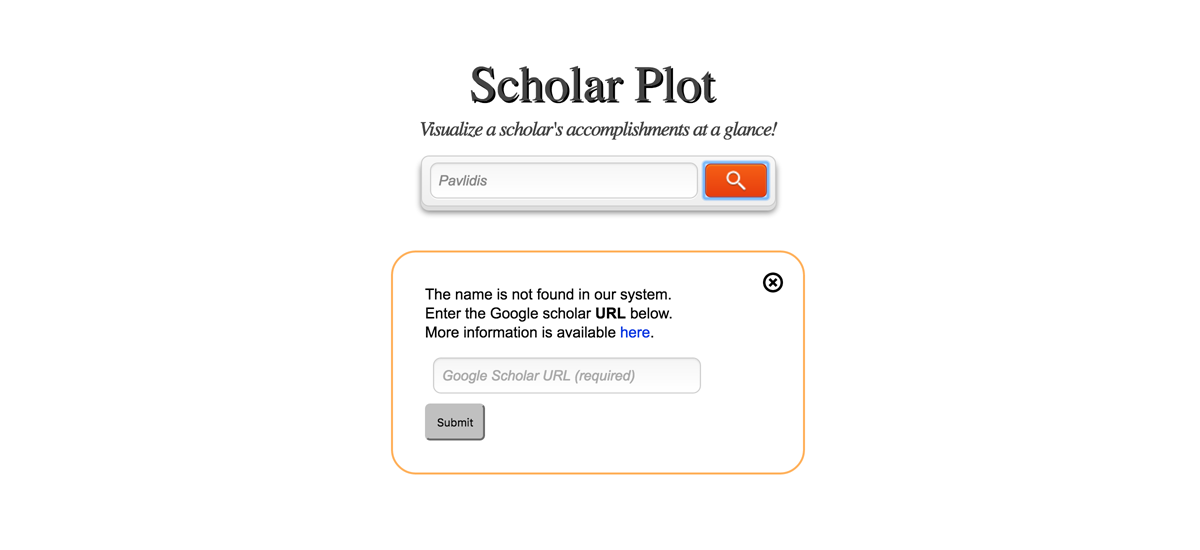
\includegraphics[width=1\textwidth]{figures/Support-4}
  \caption{Usage of Scholar Plot - No Results in Scholar Plot Search in Scholar Plot System.}~\label{fig:Support-4}
  % \vspace{-2ex}
\end{figure*}




% --------------------------
\subsection{If a name cannot be found}
% --------------------------
When a name cannot be found in our system, Scholar Plot will prompt the user to enter the URL of the person's Google Scholar Citations Profile. This URL can be found using the search bar on the Google Scholar website (\href{https://scholar.google.com/citations?mauthors=&hl=en&view_op=search_authors}here).

If the names of more than one scholar match the query, you will need to locate the correct scholar in the search results.



% --------------------------
\subsection{Google Scholar Author Search Results}
% --------------------------
From the person's Google Scholar Citations Profile page, copy the URL from your web browser's address bar.

\begin{figure*}
  \centering
  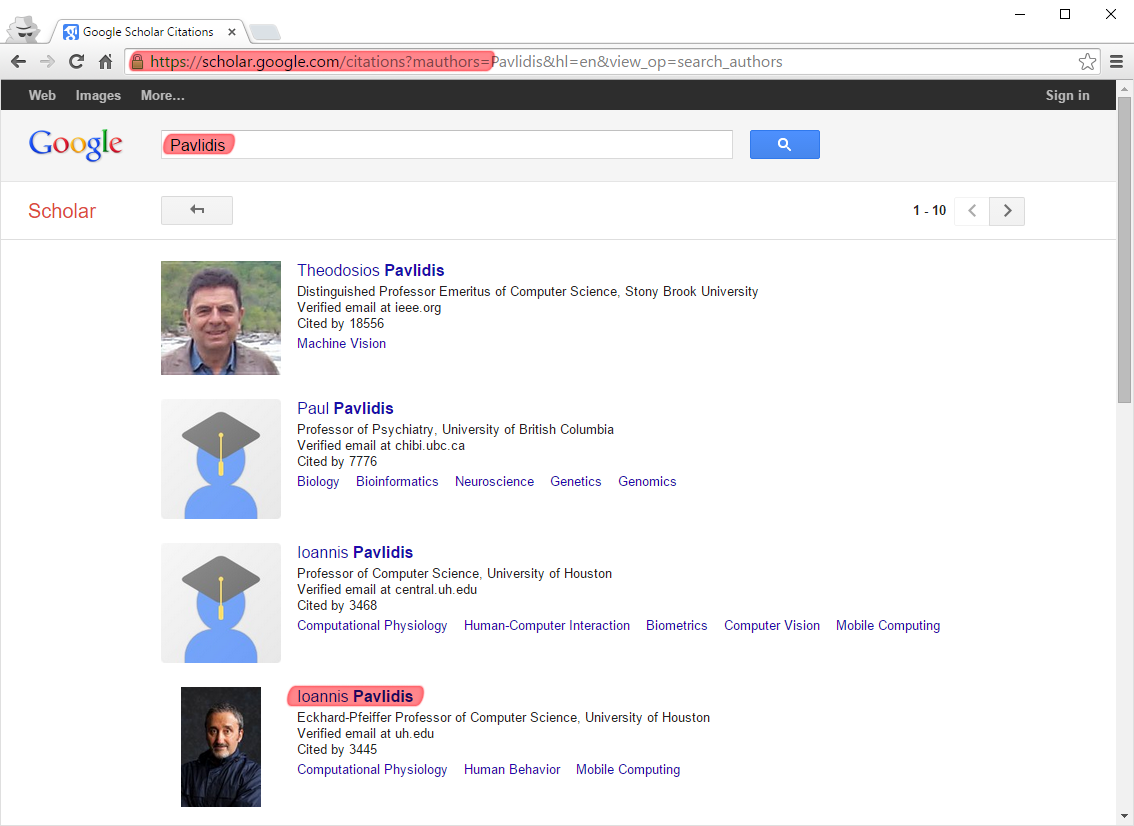
\includegraphics[width=1\textwidth]{figures/Support-1}
  \caption{Usage of Scholar Plot - Searching a scholar profile in Google Scholar.}~\label{fig:Support-1}
  % \vspace{-2ex}
\end{figure*}




% --------------------------
\subsection{Obtaining the Google Scholar Profile URL}
% --------------------------
Return to Scholar Plot and click the `Submit' button. The scholar's information will then appear and their name can be used in future searches on Scholar Plot and Scholar Compare.

\begin{figure*}
  \centering
  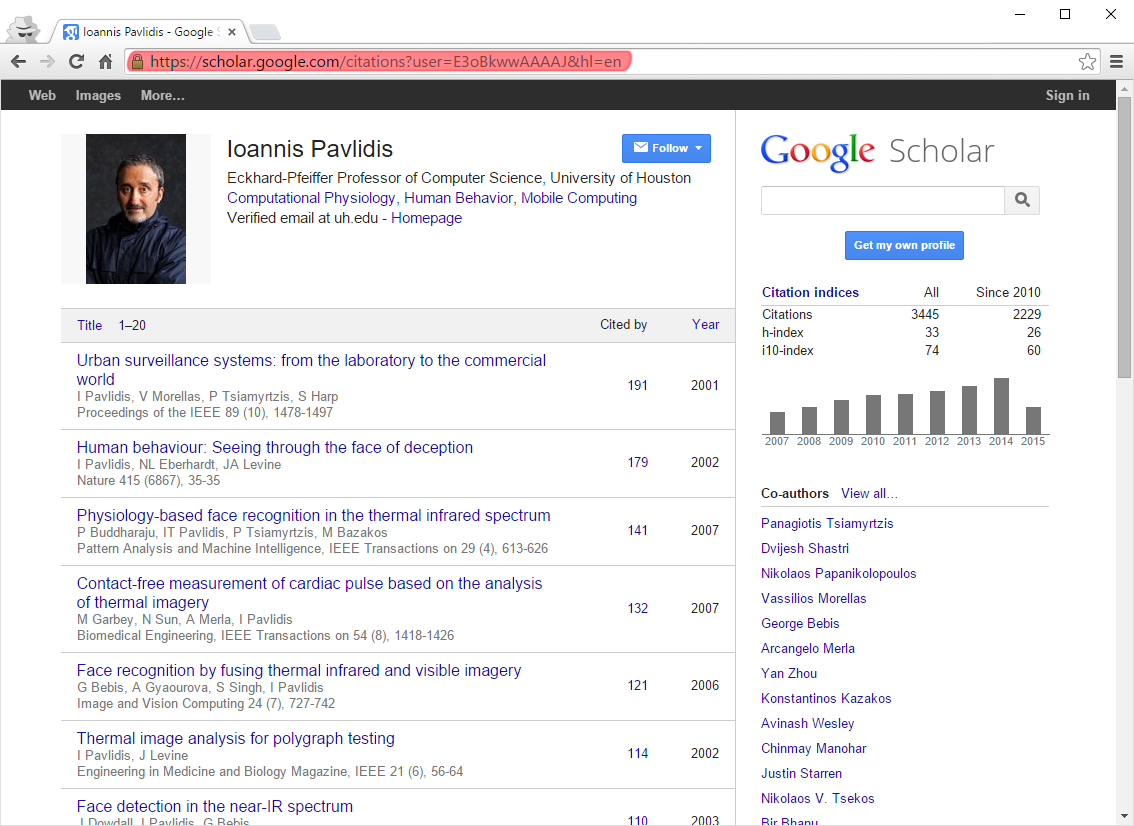
\includegraphics[width=1\textwidth]{figures/Support-2}
  \caption{Usage of Scholar Plot - Copying the Google Scholar Citations Profile URL.}~\label{fig:Support-2}
  % \vspace{-2ex}
\end{figure*}

\begin{figure*}
  \centering
  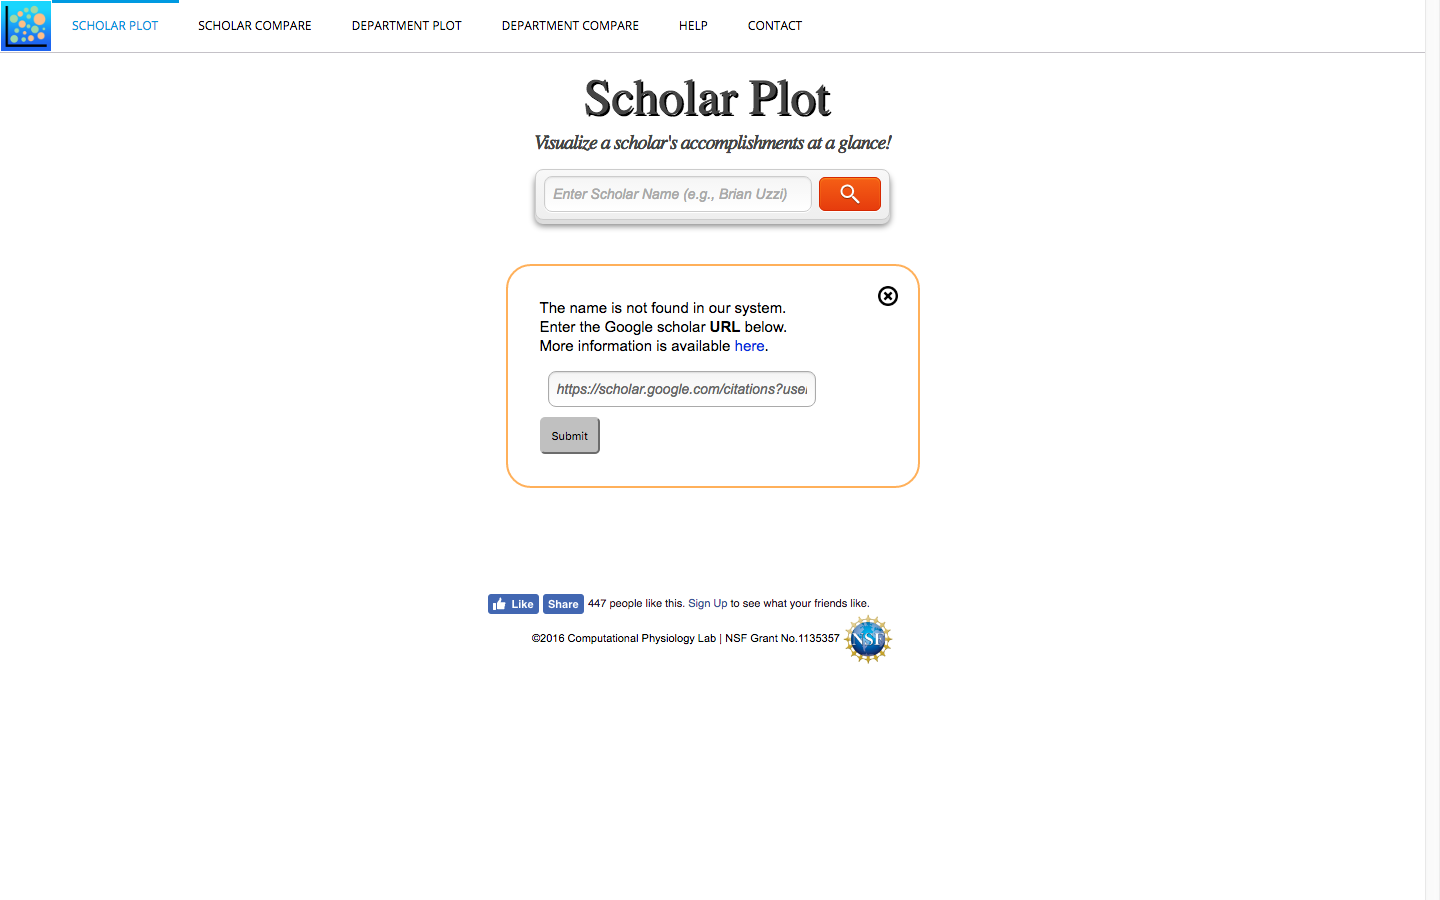
\includegraphics[width=1\textwidth]{figures/fig-paste}
  \caption{Usage of Scholar Plot - Pasting the Google Scholar Citations Profile URL.}~\label{fig:Support-5}
  % \vspace{-2ex}
\end{figure*}